\chapter{Tecnologie Utilizzate}
\pagestyle{plain}


\section{Realtà Mista (MR)}

\subsection{Storia}
Lo studio di tecnologie simili a realtà aumentata (AR), realtà mista (MR) e realtà virtuale (VR) risalgono alla fine degli anni '50, in particolare nel 1957 Morton Heiling sviluppò un simulatore, grande quanto un cabinato per videogiochi, che permetteva all'utilizzatore di visualizzare immagini 3d stereoscopiche, integrando l'esperienza con vento artificiale, vibrazioni, audio stereo e addirittura un dispositivo per la creazione di profumi.\\Ma l'applicazione che si avvicina di più a qualcosa di moderno arriva dall'utilizzo in aviazione, in particolare un sistema chiamato "Sword of Democles", un primo casco dotato di lenti per l'AR. Questo dispositivo serviva ad aiutare i piloti di elicottero ad atterrare di notte azionando le telecamere con l'utilizzo della testa. Un problema di questo dispositivo era il peso eccessivo, e da questo deriva proprio il suo nome. \\ Lo sviluppo continua nel 1992 con Loui B. Rosenberg con lo sviluppo del primo sistema AR immersivo che permetteva di guidare bracci robotici, tecnologia successivamente utilizzata nell'aereounatica militare statunitense. \cite{OverviewofAugmentedReality}
\\ In tempi recenti abbiamo visto lo sviluppo dei Google Glass, usciti nel 2013 e ritirati dal mercato nel 2023 \cite{EndofGoogleGlass}, e dei primi visori di realtà virtuale come l'Oculus Rift CV1, uscito nel 2016 \cite{OculusRift1}, che hanno creato le basi per visori più recenti come il Meta Quest 3 e gli Hololens 2, quest'utimi utilizzati proprio per la realizzazione di questa tesi.

\subsection{Definizione}
La realtà mista consente di sovrapporre al mondo fisico elementi tridimensionali con il quale l'utente può interagire. La realtà mista si contraddistingue per il fatto di avere un dispositivo, di solito un visore, che riconosce l'ambiente circostante mappandolo tridimensionali, in cui inserire oggetti tridimensionali tramite l'utilizzo di appositi sensori, la comprensione dei movimenti delle mani, degli occhi e la comprensione di input vocali.
\begin{figure}[H]
    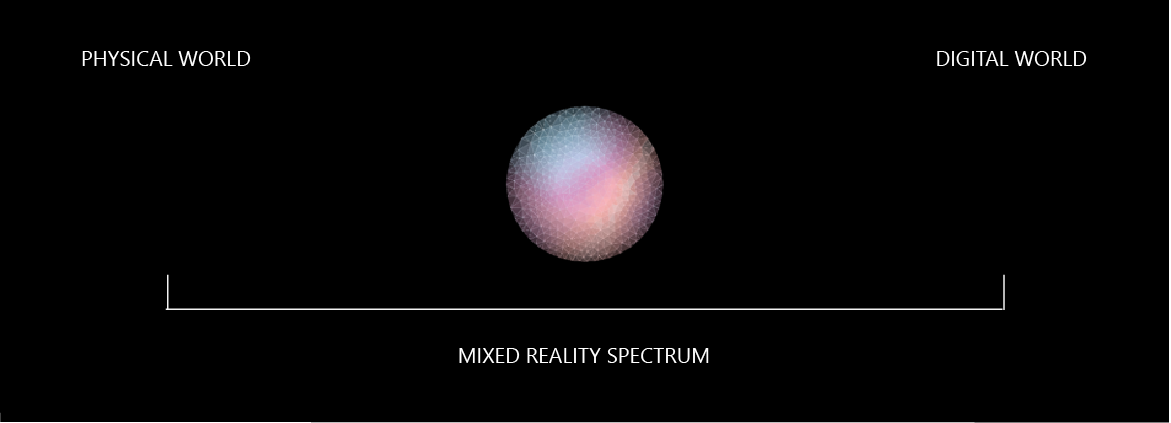
\includegraphics[scale=0.4]{figures/chapter_1/mixedrealityspectrum-worlds.png}
    \caption{Rappresentazione della fusione del mondo fisico con il mondo digitale nella realtà mista.}
    \centering
\end{figure}

Per consentire una esperienza immersiva fra realtà e oggetti 3d, chiamati anche ologrammi in ambito Microsoft, è emersa una nuova disciplina chiamata "HIC" o anche "Human-Computer Interaction", che si occupa di studiare come interagire virtualmente con il computer, ad esempio tramite tastiere, mouse, comandi vocali o tracciamenento dei movimenti. \cite{MixedRealityDefinition}

\begin{figure}[H]
    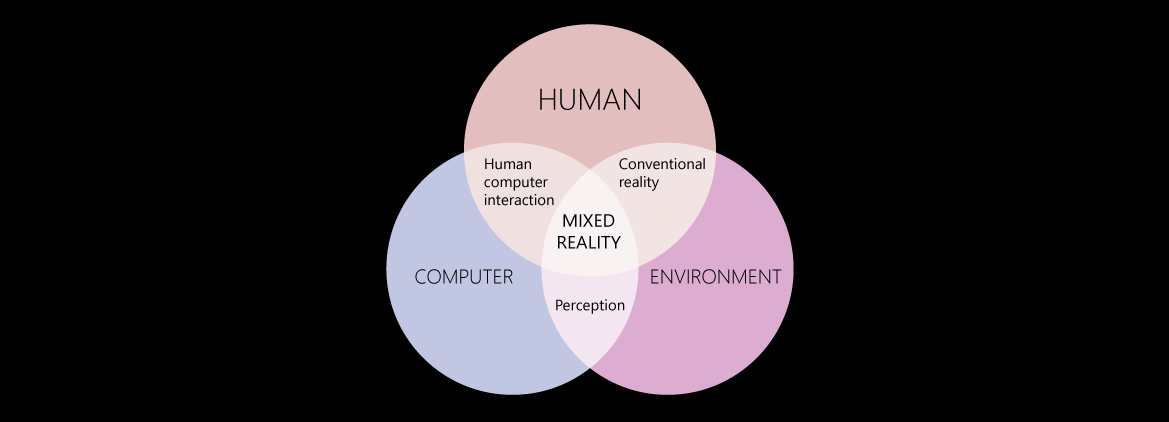
\includegraphics[scale=0.4]{figures/chapter_1/mixed-reality-venn-diagram.png}
    \caption{interazioni tra computer, utente e ambiente circostante.}
    \centering
\end{figure}
    
\subsection{Casi d'uso}
\subsubsection{Formazione di piloti in aereounatica}
Tramite l'utilizzo della realtà mista è possibile fare delle lezioni interattive simulate, ad esempio la risoluzione di un guasto all'impianto elettrico visualizzando in realtà mista la schematica dell'impianto, oppure illustrare ed allenare ad un'ispezione esterna dell'aereo. In questo ultimo caso lo studente, in una stanza abbastanza grande, può camminare intorno al modello 3d in scala dell'aereo, venendo aiutato dalla applicazione in MR durante le varie azioni di controllo, ad esempio la rotazione di maniglie o apertura di porte.\cite{MixedRealityUseCasesforPilotTraining}

\subsubsection{Formazione e simulazione in ambito industriale}
La realtà aumentata offre un modo efficace e sicuro per imparare attraverso la pratica, soprattutto in situazioni potenzialmente pericolose. Grazie a simulazioni immersive, i tirocinanti possono affrontare scenari realistici senza correre rischi reali, ricevendo feedback immediato sui propri errori. Questo tipo di formazione unisce la percezione dell'ambiante reale con l'attività virtuale, permettendo di sviluppare competenze pratiche senza creare danni a persone o macchinari \cite{MicrosoftTrainingandSimulationforEnterprises}
\begin{figure}[H]
    \centering
    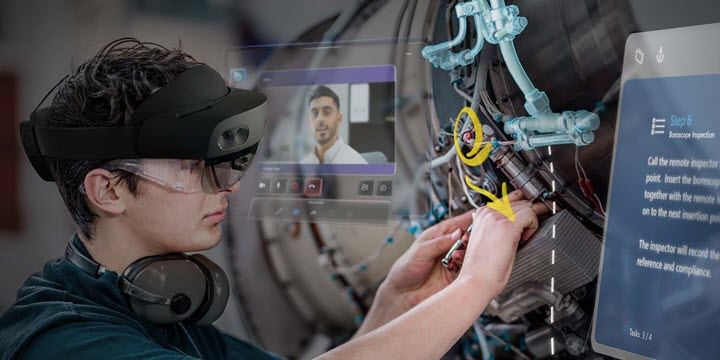
\includegraphics[width=0.5\textwidth,height=0.5\textheight,keepaspectratio]{figures/chapter_1/hololens_in_azienda.jpg}
    \caption{Utilizzo della realtà aumentata in ambito industriale}
\end{figure}

\subsubsection{Prototipazione e produzione per le imprese}
L'integrazione della realtà aumentata nei processi di prototipazione e produzione può portare a una significativa riduzione dei costi, soprattutto su scala industriale. Spostare la progettazione in uno spazio virtuale consente di evitare la produzione di prototipi fisici costosi e di velocizzare l'intero ciclo di sviluppo grazie a iterazioni rapide e meno dispendiose. Questo approccio non solo ottimizza le tempistiche, ma migliora anche la precisione nella produzione, aumentando la sicurezza e l'affidabilità delle linee produttive. In molti casi, l'introduzione della realtà aumentata ha portato benefici concreti in termini di stabilità delle infrastrutture, sicurezza dei lavoratori e qualità del prodotto finale.\cite{MicrosoftPrototypingforEnterprises}

\subsubsection{Musei e mostre virtuali}
La realtà virtuale si è dimostrata uno strumento potente per il mondo dei musei, delle mostre d'arte e d'intrattenimento, dei servizi di hosting di eventi, dei servizi turistici e di altre attività e servizi simili incentrati sulle mostre \cite{MicrosoftVirtualMuseums}. In particolare l'utilizzo della realtà mista in ambienti reali consente una perfetta armonia tra il mondo reale e quello virtuale, permettendo di visualizzare opere d'arte o reperti storici in 3d, con la possibilità di interagire con essi. \cite{MixedRealityinMuseums}

\section{Hardware}
Fra i vari visori di realtà mista, il più utilizzato è l'HoloLens 2, un visore sviluppato da Microsoft, che permette di visualizzare ologrammi in 3d e interagire con essi tramite comandi vocali, movimenti delle mani e tracciamento degli occhi. 
\subsection{HoloLens 2}
Gli HoloLens 2, successori degli HoloLens 1, sono visori di realtà mista sviluppati da Microsoft e rilasciati nel 2019, sono dotati di un display olografico che consente di sovrapporre oggetti virtuali al mondo reale e si basano sul sistema operativo "Windows Holographic OS" derivato da Windows 10

\begin{figure}[H]
    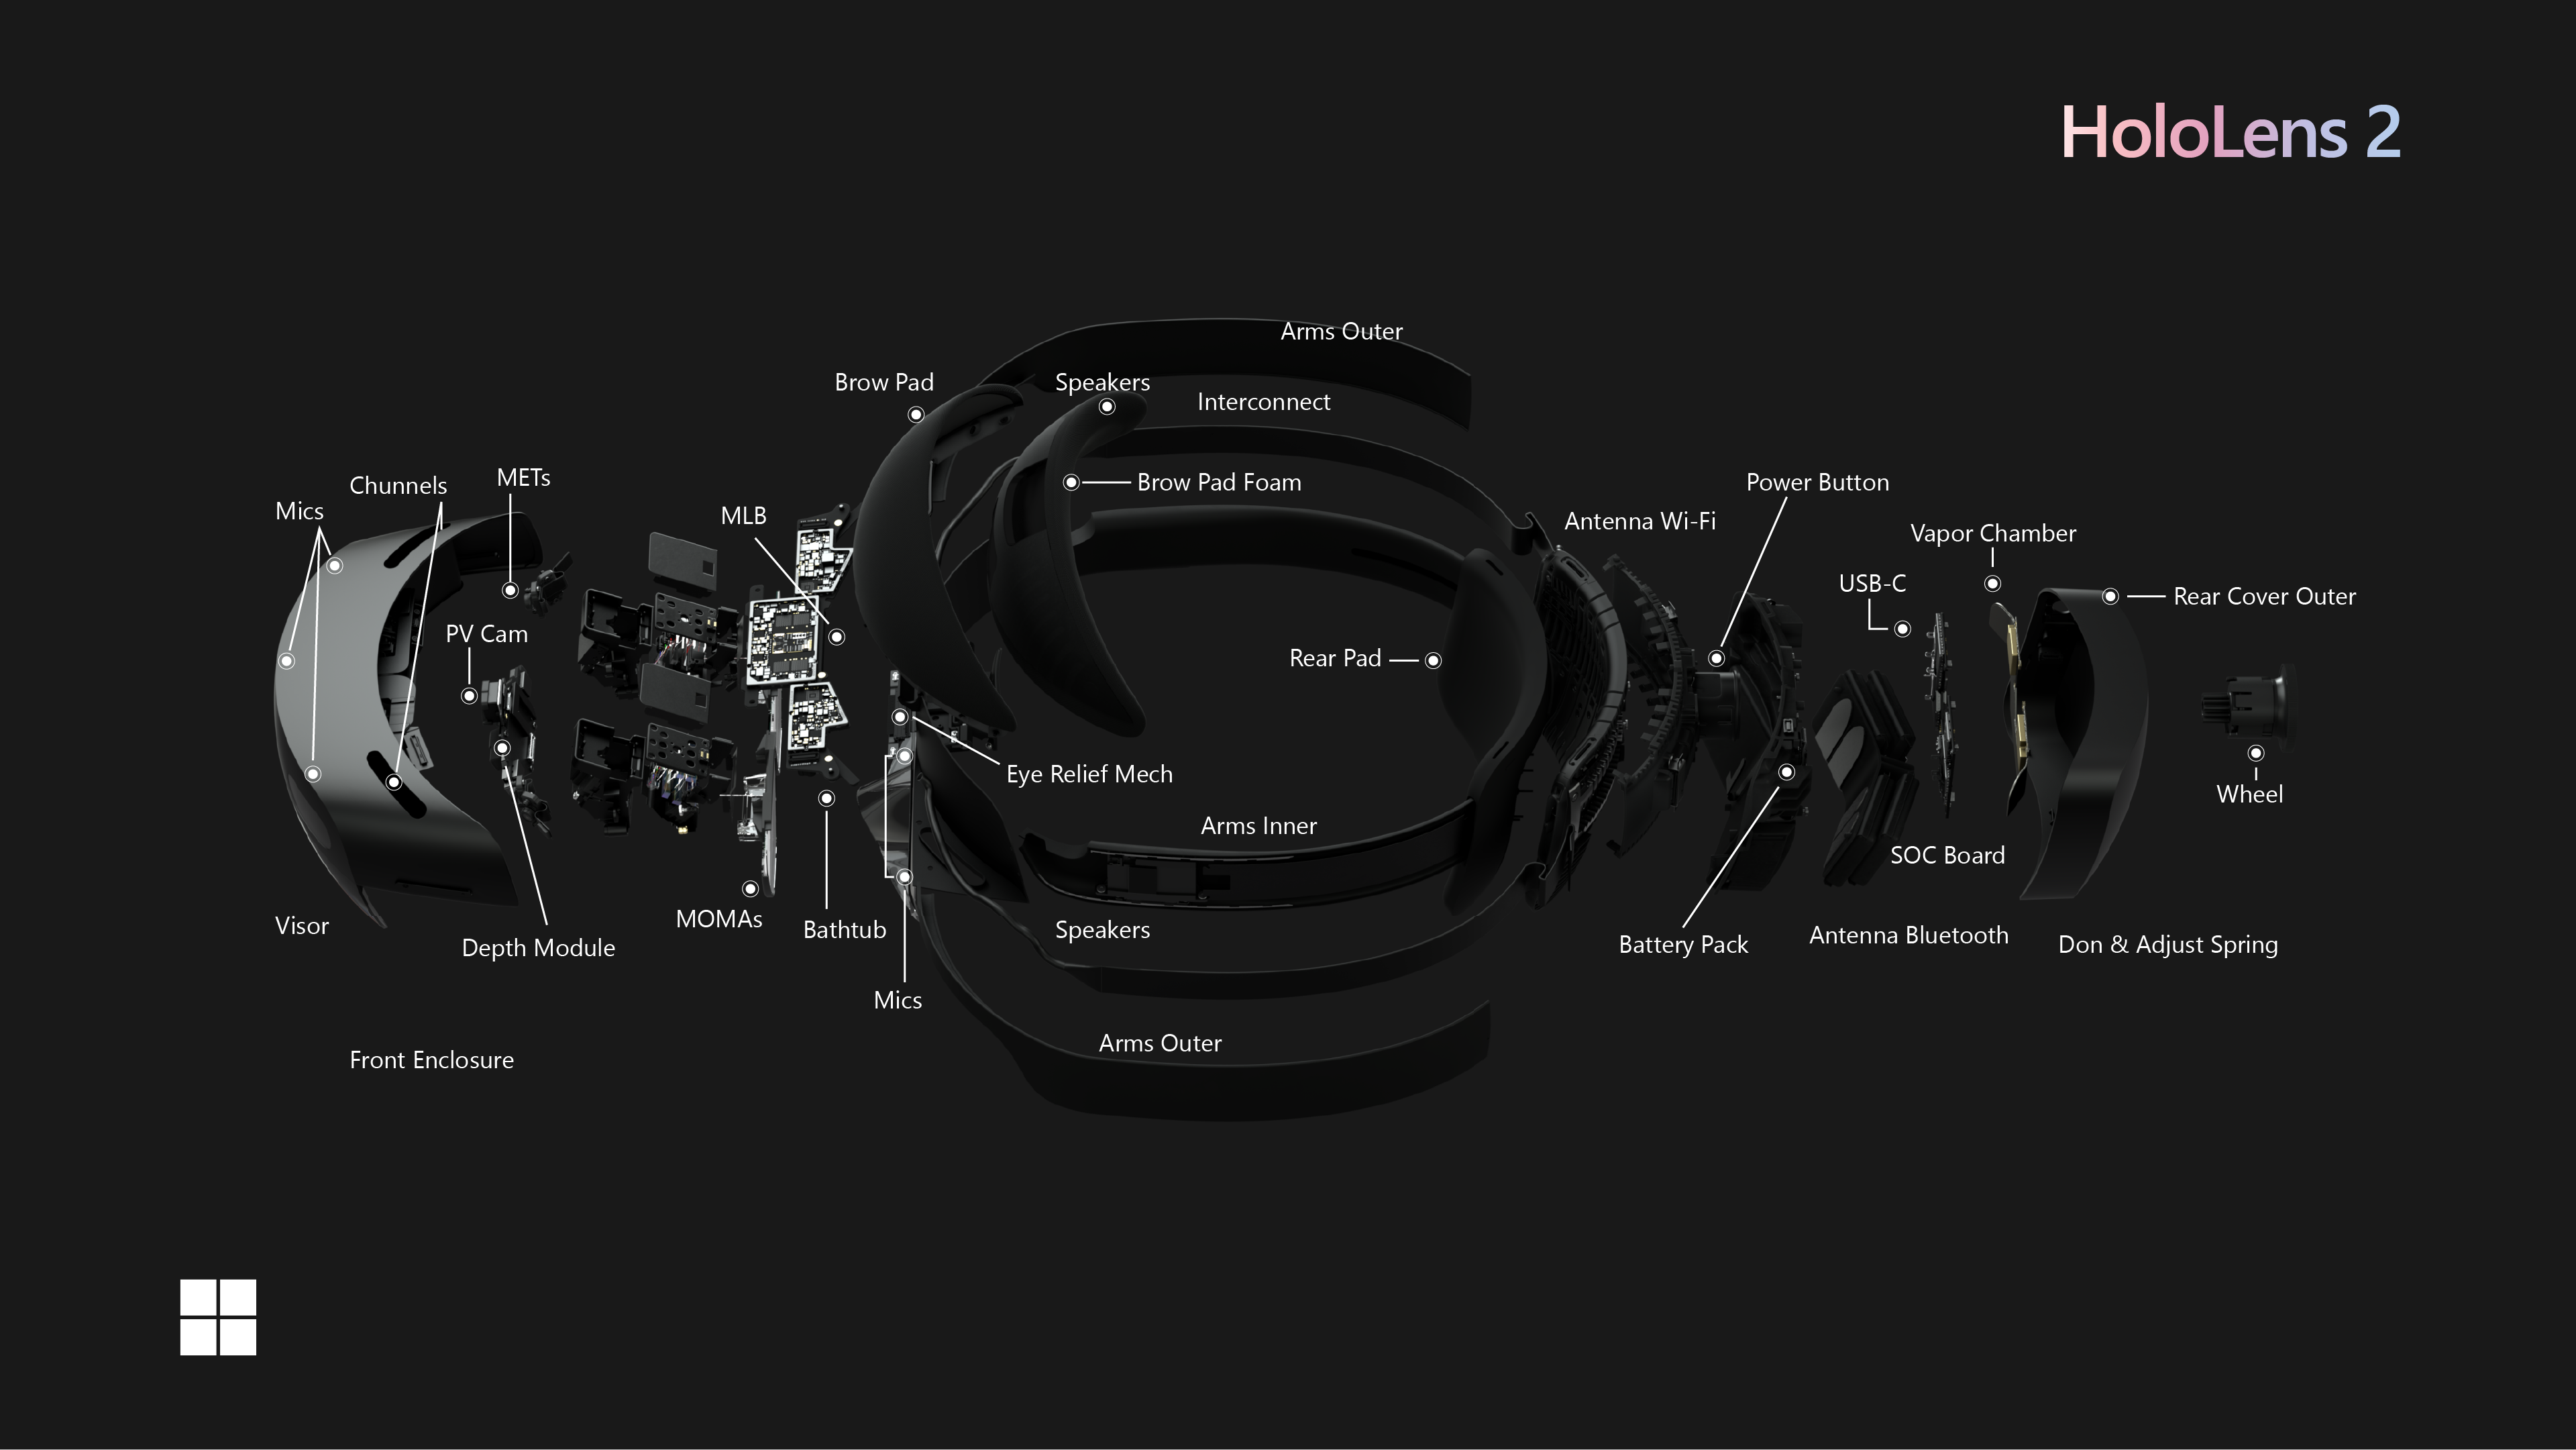
\includegraphics[width=\textwidth,height=\textheight,keepaspectratio]{figures/chapter_1/hololens2-exploded-view-diagram.png}
    \caption{Esplosione 3d del visore HoloLens 2}
    \centering
\end{figure}
Come si può vedere in figura tutta la parte di elaborazione di trova nella parte posteriore del visore, mentre nalla parte anteriore troviamo l'hardware per la proiezione degli ologrammi, i sensori come giroscopio e accelerometro, e le telecamera che permettono il tracciamento delle mani e degli occhi.In particolare abbiamo 4 telecamere frontali per il riconoscimento dell'ambiente circostante, 2 telecaere a infrarossi per il tracciamento oculare e una fotocamera frontale a colori da 8megapixel.\\
Il visore è dotato di un processore Qualcomm Snapdragon 850, 4 GB di RAM e 64 GB di memoria interna, la batteria ha una durata di circa 2-3 ore. Il visore è dotato di un sistema audio spaziale e di un microfono a 5 canali usati anche per il riconoscimento vocale. \cite{WhatIsHoloLens}\\
Per questo progetto è stato adottato questo visore solo perchè offriva l'accesso alla telecamera frontale,cosa non disponibile in altri visori come il Meta Quest 3, oltre al fatto di essere quello di più recente produzione da parte di Microsoft. 

\section{Software e AI}
Per la realizzazio del progetto sono stati utilizzati il motore grafico Unity, il Mixed Reality Toolkit (MRTK) e Google Gemini.

\subsection{Unity}
Unity è un motore grafico multipiattaforma sviluppato da Unity Technologies, utilizzato per la creazione di videogiochi e applicazioni in 2D e 3D. È particolarmente popolare per lo sviluppo di giochi per dispositivi mobili, console e PC. Nel nostro caso è stato utilizzato per la creazione di un'applicazione di realtà mista per gli HoloLens 2 utilizzando il Mixed Reality Toolkit (MRTK) e il linguaggio di programmazione C\#.
\subsubsection{Overview di Unity} 
\begin{figure}[H]
    \centering
    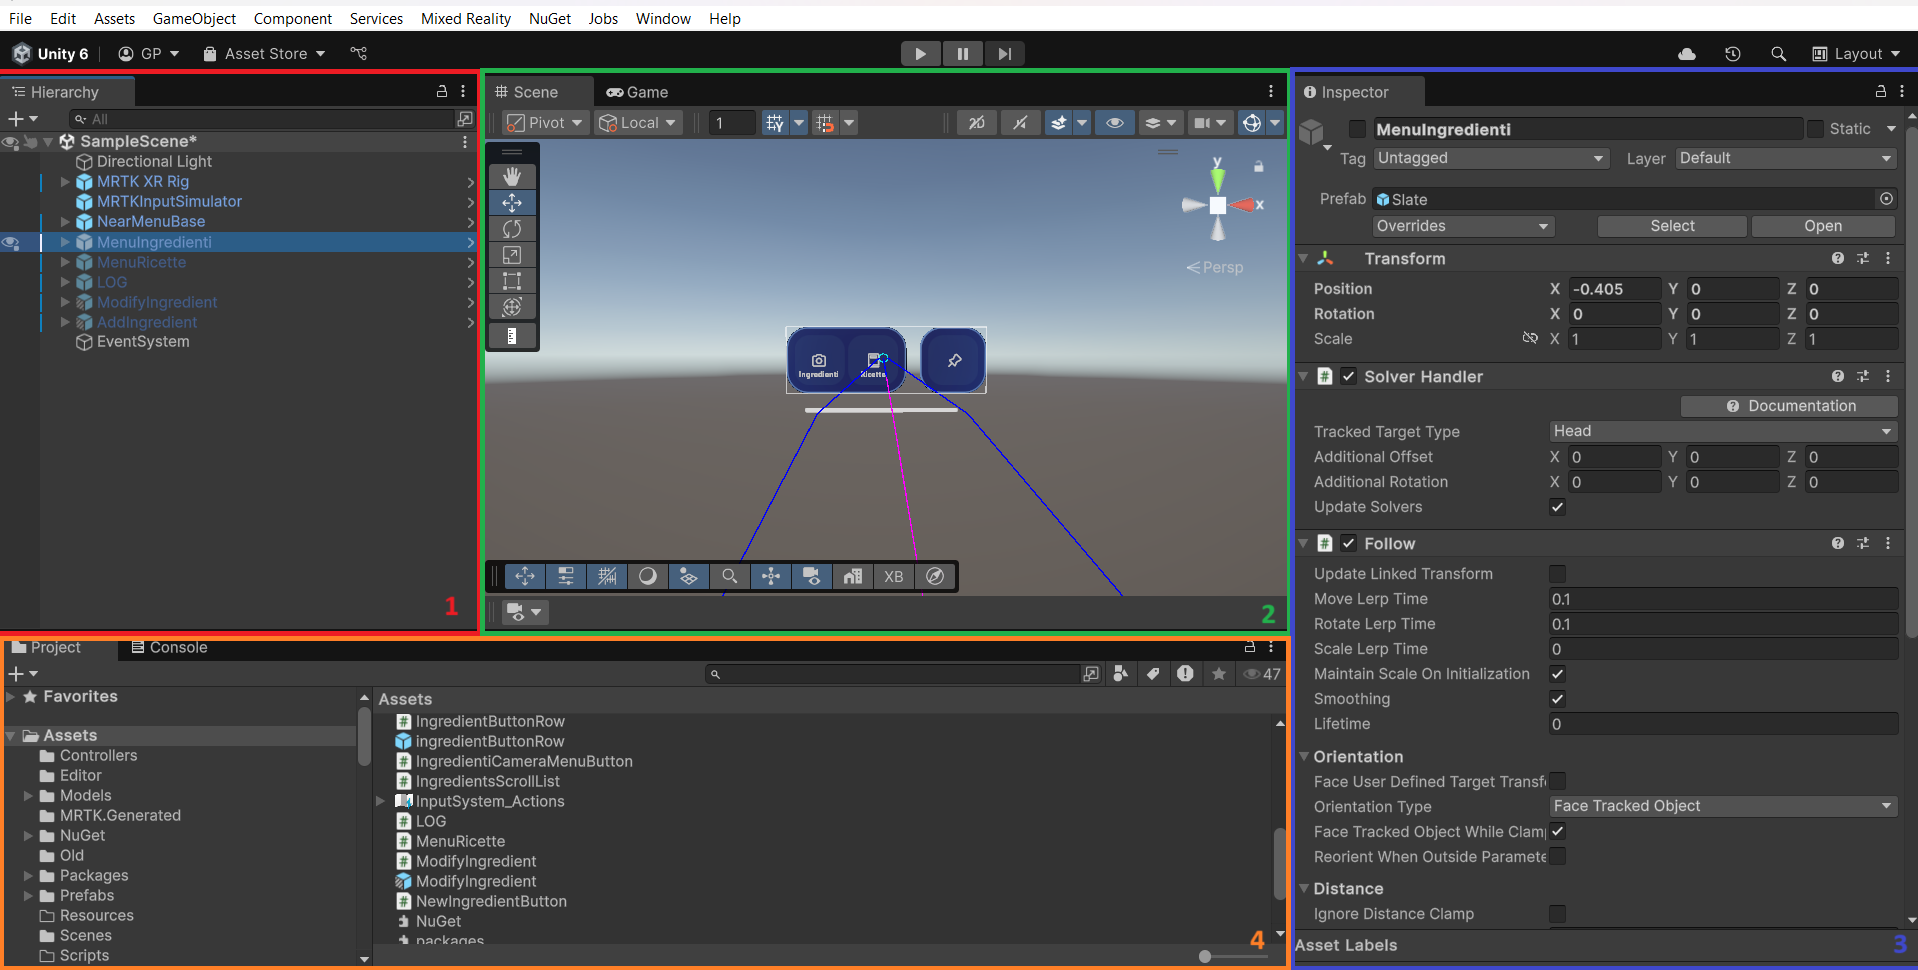
\includegraphics[width=\textwidth,height=\textheight,keepaspectratio]{figures/chapter_1/unityOverview.png}
\end{figure}
\begin{enumerate}
    \item \textbf{Gerarchia}: La gerarchia mostra tutti gli oggetti presenti nella scena. Puoi organizzare gli oggetti in una struttura ad albero, creando genitori e figli per raggruppare gli oggetti correlati.
    \item \textbf{Scena}: La scena è l'area di lavoro principale in Unity, dove puoi posizionare e organizzare gli oggetti 3D, le luci e le telecamere. Puoi visualizzare la scena in diverse modalità, come la vista 3D o la vista 2D.
    \item \textbf{Inspector}: L'Inspector mostra le proprietà e i componenti dell'oggetto selezionato nella gerarchia. Puoi modificare le proprietà degli oggetti, aggiungere componenti e configurare le impostazioni. Un componente potrebbe essere anche uno script C\# che definisce il comportamento dell'oggetto.
    \item \textbf{Project e Console}: La finestra Project mostra tutti i file e le risorse del tuo progetto, come modelli 3D, texture, suoni e script. Puoi organizzare le risorse in cartelle per una gestione più semplice. La Console mostra i messaggi di errore, avviso e debug generati durante l'esecuzione del gioco o dell'applicazione.
\end{enumerate}

\subsection{MRTK}
\begin{figure}[H]
    
\includegraphics[width=\textwidth,height=\textheight,keepaspectratio]{figures/chapter_1/logo_mrtk_unity_banner.png}
    \centering
\end{figure}
L'MRTK è un progetto della Microsoft che fornisce una serie di strumenti e librerie per lo sviluppo di applicazioni di realtà mista su piattaforme Microsoft, in particolare per gli HoloLens. Il toolkit include una serie di componenti e funzionalità per facilitare lo sviluppo di interfacce utente, il tracciamento delle mani, il riconoscimento vocale e altre funzionalità specifiche per la realtà mista. L'MRTK è progettato per essere facilmente integrato in Unity e offre una serie di esempi e documentazione per aiutare gli sviluppatori a iniziare rapidamente.\\
Oltre a supportare gli Hololens supporta anche altri visori come gli Oculus e permette anche di creare applicazioni AR (Argumented Reality) per Android e iOS.\cite{WhatIsMixedRealityToolkit}


\subsection{Google Gemini}
Google Gemini, inizialmente uscita sotto il nome di Google Bard, rappresenta uno dei più recenti sviluppi dell'intelligenza artificiale generativa di Google. Gemini, oltre a elaborare del testo, è in grado di comprendere anche immagini, audio, documenti e altri file di tipo testuale.
L'obiettivo di Google con Gemini è offrire un assistente personale basato su intelligenza artificiale che sia non solo utile e produttivo, ma anche creativo e capace di stimolare la curiosità dell'utente. In ambito produttivo, Gemini può ad esempio sintetizzare documenti lunghi, supportare attività di scrittura, aiutare nella programmazione e automatizzare attività complesse.\\
Nonostante il grande potenziale, Google riconosce che la tecnologia è ancora in una fase iniziale e presenta alcune limitazioni tipiche dei modelli linguistici di grandi dimensioni (LLM). Tra queste, vi sono il rischio di fornire risposte inaccurate, la possibilità che emergano bias nei contenuti generati, e la difficoltà nel rappresentare prospettive multiple su questioni soggettive. Inoltre, l'assistente può occasionalmente mostrare segnali di “personalizzazione” e sembrare esprimere emozioni o opinioni, che in realtà non possiede, essendo un modello statistico. Altri limiti includono i cosiddetti falsi positivi e falsi negativi, ossia casi in cui Gemini rifiuta di rispondere a domande appropriate o, al contrario, fornisce risposte inappropriate. Infine, il sistema può essere vulnerabile a prompt avversari, ovvero tentativi intenzionali di metterne alla prova i limiti o aggirarne i filtri di sicurezza.\\
Per evitare ciò, e rispettare le proprie linee guida, Google ha adottato un approccio responsabile nello sviluppo di Gemini, condudendo degli stress test svolti da team interni incaricati di individuare criticità, formando appositi "red team", composti da esperti e scienziati sociali.\cite{GeminiLaunch} \cite{GeminiAppOverview}
